% Copyright 2004 by Till Tantau <tantau@users.sourceforge.net>.
%
% In principle, this file can be redistributed and/or modified under
% the terms of the GNU Public License, version 2.
%
% However, this file is supposed to be a template to be modified
% for your own needs. For this reason, if you use this file as a
% template and not specifically distribute it as part of a another
% package/program, I grant the extra permission to freely copy and
% modify this file as you see fit and even to delete this copyright
% notice. 

\documentclass{beamer}
\usepackage{color}
\usepackage{graphicx}
\usepackage{marvosym}
\usepackage{tikz}
\setbeamertemplate{items}[circle]

\usetheme{Madrid}
\newcommand{\mc}{\mathcal}
\newcommand{\mb}{\mathbf}
\newcommand\numberthis{\addtocounter{equation}{1}\tag{\theequation}}
\let\oldnl\nl
\newcommand{\nonl}{\renewcommand{\nl}{\let\nl\oldnl}}

\DeclareMathOperator*{\argmin}{arg\,min}
\DeclareMathOperator*{\vcdim}{VC-Dim}

\newcommand\mynum[1]{%
  \usebeamercolor{enumerate item}%
  \tikzset{beameritem/.style={circle,inner sep=0,minimum size=2ex,text=enumerate item.bg,fill=enumerate item.fg,font=\footnotesize}}%
  \tikz[baseline=(n.base)]\node(n)[beameritem]{#1};%
}

\title[Clustering for de-dup]{Semi-supervised clustering for de-duplication}

\author[Kushagra]{
Shrinu Kushagra\\
\vspace{30pt}Joint work with\\ Hemant Saxena, Ihab Ilyas and Shai Ben-David\\
University of Waterloo
}
\date{\today}

\AtBeginSubsection[]
{
  \begin{frame}<beamer>
  \frametitle{Outline}
    \tableofcontents[currentsection]
  \end{frame}
}

% Let's get started
\begin{document}

\begin{frame}
  \titlepage
\end{frame}

\begin{frame}{What is data de-duplication?}
	Consider a database $X$ with records (or rows) $r_1, \ldots, r_n$\\
    \vspace{20pt}``Detect'' records which correspond to the same real-world entity. \\
    \vspace{30pt}Central task in \textit{cleaning} large databases.
\end{frame}

\begin{frame}{De-duplication}
	\onslide<1->
    Detecting records could mean.
    \begin{itemize}
    	\item Output a list of pairs where each pair is a duplicate.
    \end{itemize}
    
    \onslide<2->
    \vspace{20pt}Our view is to output
    $$C = \{C_1, \ldots, C_k \}$$
    where $C_i \cap C_j = \phi$ and $\cup C_i = X$.
    
    \vspace{30pt}Output a clustering of $X$.
    \begin{itemize}
    	\item Records corresponding to the same entity share a cluster.
    	\item Records corresponding to different entities are separated.
    \end{itemize}
\end{frame}

\begin{frame}{Clustering for de-duplication}
	Challenges\\
    \begin{itemize}
    	\vspace{20pt}\item Standard techniques like $k$-means, $k$-median etc. are not suitable.\\
    	\textcolor{blue}{$k$ is unknown.}
	\end{itemize}    	
\end{frame}

\begin{frame}{Correlation clustering (CC) for de-duplication}
	Input: Graph $G = (V, E)$. Edges are labelled $1$ and $0$\\
    \vspace{20pt}Find a clustering which minimizes
    
    \begin{center}
    \textcolor{blue}{\# zero edges within a cluster + \# one edges\\ across different clusters}
    \end{center}
    
    \vspace{20pt}Edge labelling can be \textit{inferred} from a distance metric $d$ over $X^2$.
\end{frame}

\begin{frame}{CC framework: Missing pieces}
	Agnostic to some information ``stored" in the metric $d$ (or the edges $E$)
    \begin{itemize}
    	\vspace{10pt}\item If $E$ corresponds to a clustering, then finding that clustering is easy.\\
    	\vspace{10pt}\item What if the optimal solution is `close to' $E$ ? 
	\end{itemize}
	
	\onslide<2->
	\vspace{20pt}Applicability of human supervision
	\begin{itemize}
    	\vspace{10pt}\item Given two records $r_1$ and $r_2$, do they correspond to the same or different real-world entity?.\\
    	\item Such \textit{same-cluster} queries can be answered by a human with a high degree of accuracy.
	\end{itemize}
\end{frame}

\begin{frame}{Promise Correlation Clustering (PCC)}
	\begin{block}{Input}
		$G = (X, E)$
	\end{block}
	
	\begin{block}{Find}
	\vspace{-15pt}\begin{align*}
	  &C^* = \argmin_{C \in \mc F} \enspace \text{correlation-loss}_{E}(C) \label{eqn:promiseCorrLoss}
	\end{align*}
	
	where $\mc F$ is the set of all possible clusterings $C$ such that maximum size of a cluster of any clustering in $\mc F$ is atmost $M$. 
	\end{block}
	
	\begin{block}{Given}
		$E$ is $(\alpha, \beta)$-informative
		\vspace{-10pt}\begin{align*}
			&\underset{(x, y) \sim U^2}{\mb P}\enspace \big[ (x, y) \not\in E \enspace|\enspace C^*(x, y) = 1\big] \enspace \le \enspace \alpha \\
			&\underset{(x, y) \sim U^2}{\mb P}\enspace \big[C^*(x, y) = 1 \enspace|\enspace (x, y) \in E \big] \enspace \ge \enspace \beta 
		\end{align*}
	\end{block}	
\end{frame}


\begin{frame}{PCC is NP-Hard}
	\begin{block}{Theorem}
		Finding the optimal solution to the Promise Correlation Clustering problem is NP-Hard for all $M \ge 3$ and for $\alpha = 0$ and $\beta = \frac{1}{2}$.  
	\end{block}
	
	\onslide<2->
	\vspace{10pt}Reduction from Exact Cover by $3$-sets (X3C).
	\begin{itemize}
		\vspace{10pt}\item Given a universe of elements $ U= \{x_1 , \ldots, x_{3q} \}$.
		\item A collections of subsets $S = \{S_1 , \ldots, S_m \}$. Each $S_i \subset U$ and $|S_i| = 3$
		\item Does there exist $S' \subseteq S$ such that each element of $U$ occurs
exactly once in $S'$ ?
	\end{itemize}
\end{frame}

\begin{frame}{Hardness of PCC}
	\begin{columns}
		\begin{column}{0.48\textwidth}
			\vspace{-40pt}\begin{figure}
				\centering
				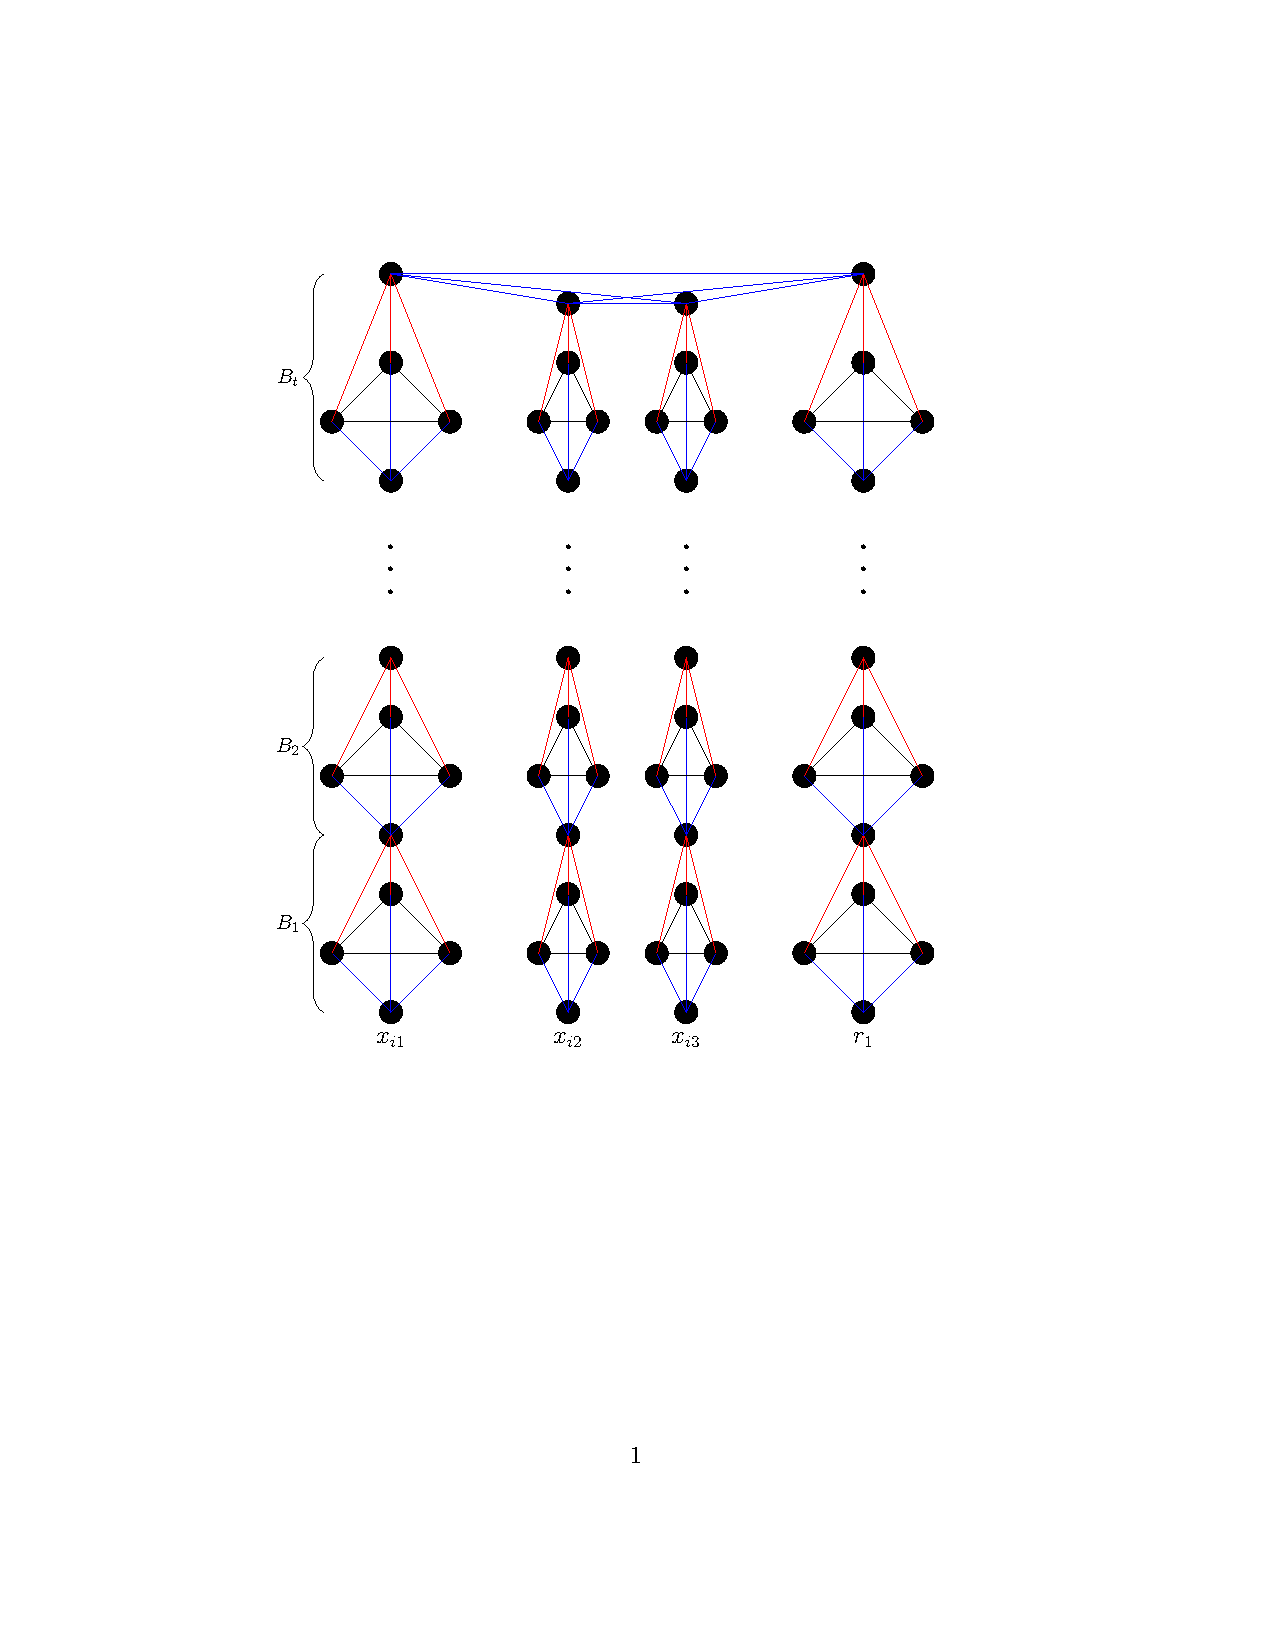
\includegraphics[trim = 100 290 100 100, clip, width=6cm, height=4.5cm]{figures/deDuplication/pccHard.pdf}
			\end{figure}
		\end{column}

		\begin{column}{0.48\textwidth}
		    Part of graph $G$ constructed by local replacement for the subset $S_i =  \{x_{i1}, x_{i2}, x_{i3}\}$. Illustration for $M = 4$.
		\end{column}
	\end{columns}

	
	\vspace{10pt}\begin{itemize}
		\item If $A$ outputs a clustering such that all clusters have size $M$ and no negative erros, then output YES.
		\item Else NO.
	\end{itemize}
\end{frame}

\begin{frame}{CC framework: Missing pieces}
	Two options
	\begin{enumerate}
		\item Adding information ``stored" in the the edges $E$
		\vspace{10pt}\item Adding human supervision
	\end{enumerate}
	
	\vspace{20pt}Proved that
	\begin{enumerate}
		\item alone doesn't help (just proved)
		\vspace{10pt}\item alone doesn't help (proved by others)
	\end{enumerate}
	
	\vspace{20pt}How about \mynum{1} and \mynum{2}?
\end{frame}

\begin{frame}{Hardness of PCC in the presence of an oracle}
	\begin{block}{Theorem}
		Given that the Exponential Time Hypothesis (ETH) holds. Any algorithm for PCC that runs in polynomial time makes $\Omega(|X|)$ same-cluster queries for all $M \ge 3$ and for $\alpha = 0$ and $\beta = \frac{1}{2}$. 
	\end{block}
	
	\onslide<2->
	\vspace{20pt}Strategy: Any algorithm for PCC takes $2^{\Omega(n)}$ time.
	\begin{itemize}
		\item Any algorithm for X3C or equivalently 3DM takes $2^{\Omega(m)}$ time.
	\end{itemize}
	
	\begin{block}{3DM}
		\textbf{Input}: Sets $W, X$ and $Y$ and a set of matches $M \subseteq W \times X \times Y$ of size $m$.  \\
		\textbf{Output}: YES if there exists $M' \subseteq M$ such that each element of $W, X, Y$ appears exactly once in $M'$. \\
		NO otherwise. 
	\end{block}
\end{frame}

\begin{frame}{Hardness: Linear reduction of 3SAT to 3DM}
	\begin{columns}
		\begin{column}{0.48\textwidth}
			\vspace{-40pt}\begin{figure}
				\centering
				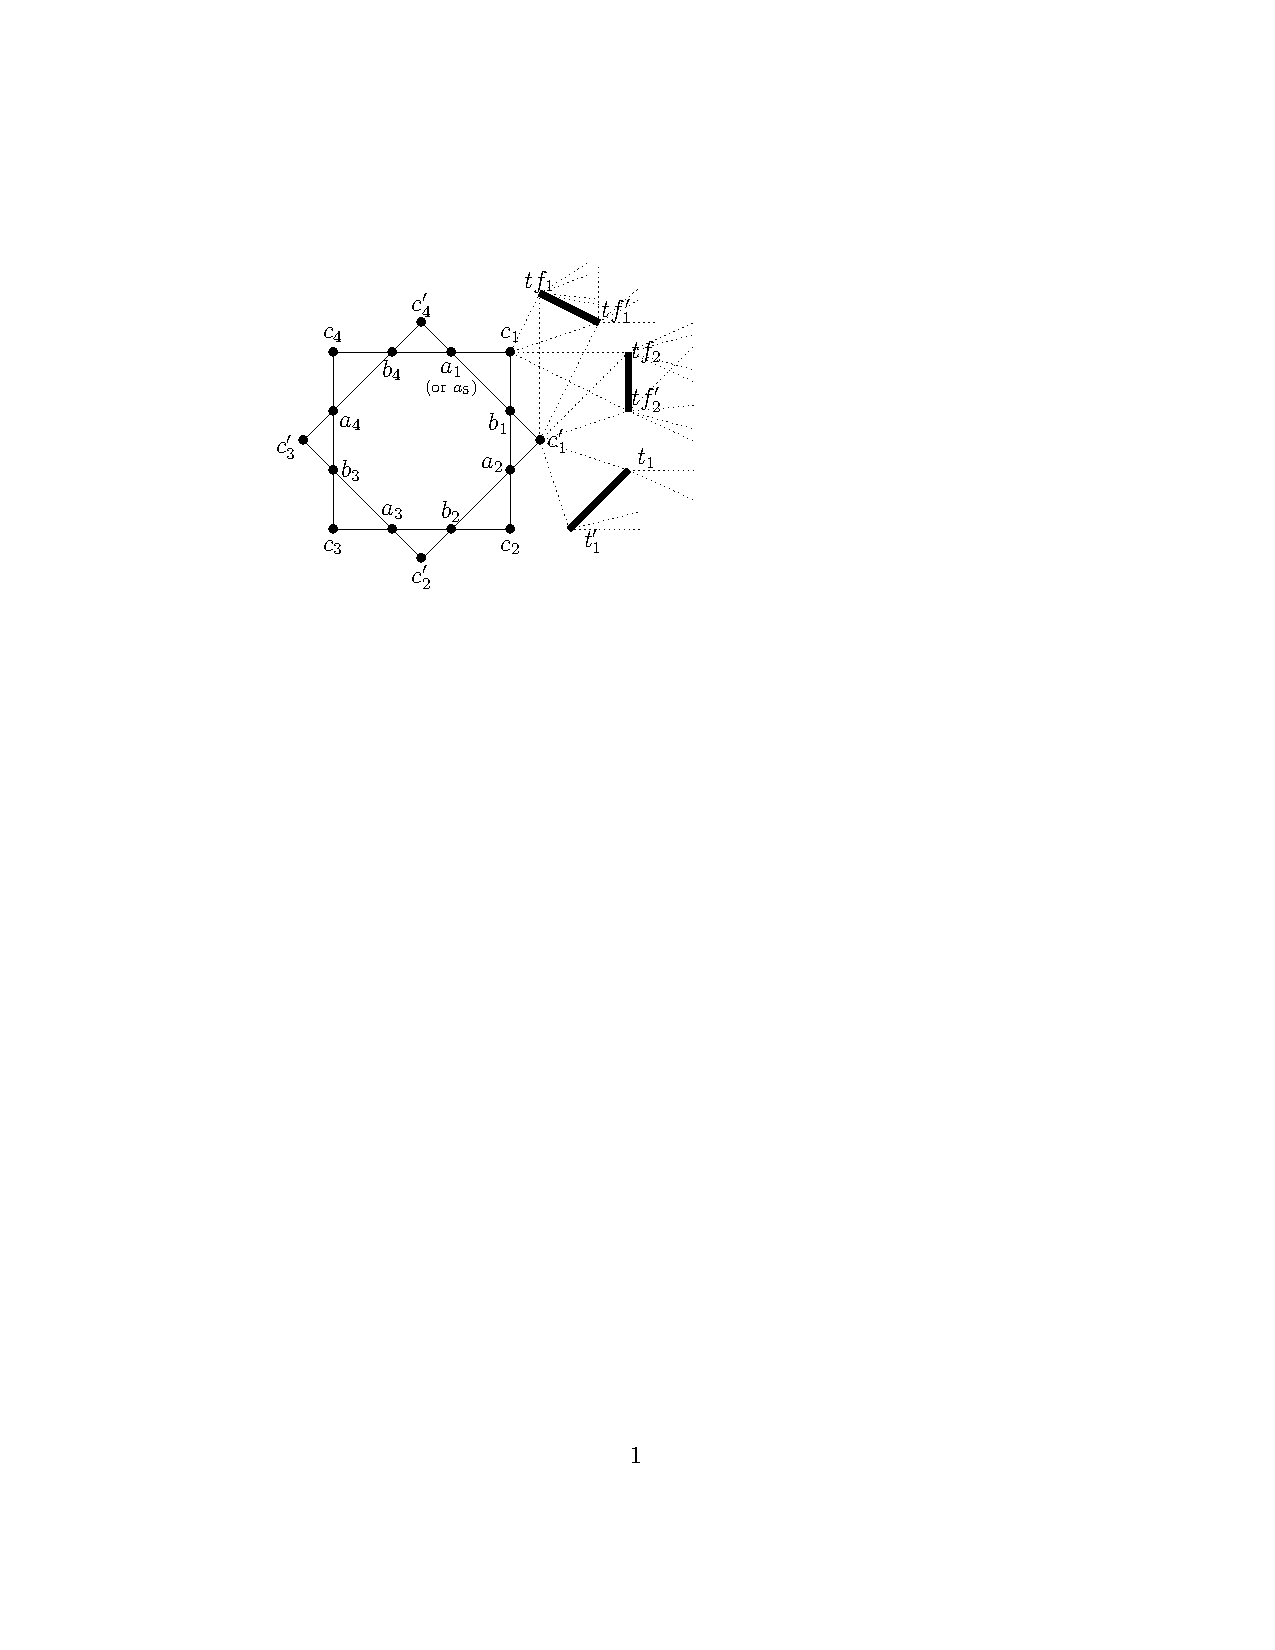
\includegraphics[trim = 120 500 300 120, clip, width=\linewidth]{figures/deDuplication/pccHardQuery.pdf}
			\end{figure}
		\end{column}

		\begin{column}{0.48\textwidth}
			\begin{itemize}
				\item Literal $x_1$ is part of four different clauses.
				\item $(a_i, b_i, c_i)$ capture truth assignment and $(b_i, c_i', a_{i+1})$ captures false assignment.
				\item Hyper-edges containing $tf_i, tf_i'$ and $t_1, t_1'$ capture truth setting for the clause $C = \{x_1, x_2, x_3\}$.
				
			\end{itemize}
		\end{column}
	\end{columns}	
	\begin{itemize}
		\item $t_1, t_1'$ ensure that atleast one of the literals is true. 
	\end{itemize}
\end{frame}

\begin{frame}
    \Huge{
    \begin{center}
    	Disappointing !!\\
    	\Frowny{} 
   	\end{center}
    }
\end{frame}

\begin{frame}{Circumventing the hardness?}
	Possible approach
	\begin{itemize}
		\item Design efficient approximation algorithms.		
	\end{itemize}
	
	\onslide<2->
	\vspace{30pt}Our approach
	\begin{itemize}
		\vspace{5pt}\item Limit the search space of clusterings $\mc F$.
		\vspace{5pt}\item Choose the best from a class of clusterings (or algorithms).
		\vspace{5pt}\item Useful tool for practitioners. 
	\end{itemize}
\end{frame}

\begin{frame}{Problem formulation: Attempt 1}
	Input: $G = (X, E)$ and a class of clusterings $\mc F$\\
	
	\vspace{10pt}Output: 
	\vspace{-10pt}\begin{align*}
	  &\hat C = \argmin_{C \in \mc F} \enspace \text{correlation-loss}_{E}(C)
	\end{align*}
	
	\onslide<2>
	Solution: 
	\begin{itemize}
		\item Iterate over clusterings in $\mc F$		
		\item Choose the one with smallest loss.
	\end{itemize}
\end{frame}


\begin{frame}{Restricted Correlation Clustering (RCC)}
	\begin{block}{Input}
		$(X, d)$, class of clusterings $\mc F$ and a $C^*$-oracle
	\end{block}
	
	\vspace{10pt}\begin{block}{Find}
		\vspace{-15pt}\begin{align*}
		  &\hat C = \argmin_{C \in \mc F} \enspace \text{correlation-loss}_{C^*}(C)
		\end{align*}	
	\end{block}
	
	\begin{block}{where}
		\vspace{-20pt}\begin{align*}
			d \text{ is }(\alpha, \beta)\text{-informative}&\\
			\text{correlation-loss}_{C^*}(C) &= \enspace  \mu \enspace \underset{(x, y) \sim P^+}{\mb P} \big[ C(x, y) = 0 ] \\
			&+\enspace (1-\mu) \enspace \underset{(x, y) \sim P^-}{\mb P} \big[ C(x, y) = 1] 
		\end{align*}
	\end{block}	
	$P^+$ is the uniform distribution over pairs where $C^*(x, y) = 1$
\end{frame}


\begin{frame}{Solution Strategy}
	\begin{block}{Algorithm}
		\begin{itemize}
			\vspace{10pt}\item Sample `enough' positive pairs.
			\vspace{10pt}\item Sample `enough' negative pairs.
			\vspace{10pt}\item Estimate correlation loss of each $C \in \mc F$.
			\vspace{10pt}\item Output clustering with minimum loss.
		\end{itemize}
	\end{block}
	
	\vspace{20pt}Uniform sampling doesn't work\\
	\vspace{10pt}Make use of informative metric $d$
\end{frame}

\begin{frame}{Sampling negative pairs}
	
	\vspace{10pt}\textcolor{blue}{Basic Idea}\\
	Sample (with rejection) uniformly at random from $X^2$. 
	
	\vspace{20pt}\begin{block}{Results}
		The above procedure
		\begin{itemize}
			\item Samples a pair according to $P^-$.
			\item Makes $\frac{1}{1-\gamma}$ queries to the oracle in expectation. 
		\end{itemize}			
	\end{block}
	
	
\end{frame}

\begin{frame}{Sampling positive pairs}
	Recall the definition of $(\alpha, \beta)$-informative metric
	\vspace{-10pt}\begin{align*}
		&\underset{(x, y) \sim U^2}{\mb P}\enspace \big[d(x, y) > \lambda \enspace|\enspace C^*(x, y) = 1\big] \enspace \le \enspace \alpha \\
		&\underset{(x, y) \sim U^2}{\mb P}\enspace \big[C^*(x, y) = 1 \enspace|\enspace d(x, y) \le \lambda \big] \enspace \ge \enspace \beta
	\end{align*}

    
	\vspace{20pt}\textcolor{blue}{Basic Idea}\\
	Sample (with rejection) uniformly at random from $K = \{(x, y): d(x, y) \le \lambda\}$. 
\end{frame}

\begin{frame}{Sampling positive pairs}

	\begin{block}{Results}
		The above procedure
		\begin{itemize}
			\item Samples a pair according to distribution $T$ which approximates $P^+$.
			$$\Big|\underset{(x, y) \sim P^+}{\mb P}\enspace \big[ h(x, y) = 0 ] - \underset{(x, y) \sim T}{\mb P}\enspace \big[ h(x, y) = 0 ]\Big|  \enspace \le \enspace 2\alpha.$$ 
			The loss computed according to $T$ is similar to loss computed according to $P^+$ for any labeling function.
			\item Makes $\frac{1}{\beta}$ queries to the oracle in expectation. 
		\end{itemize}			
	\end{block}
	
\end{frame}

\begin{frame}{Recap}
Procedure to sample $m_+$ positive pairs.\\
\vspace{20pt}Procedure to sample $m_-$ negative pairs.\\
\vspace{20pt}Estimate the loss from this sample.
\end{frame}

\begin{frame}{Positive result}
	\begin{block}{Sample complexity}
		If the number of positive and negative samples   
		\vspace{-10pt}\begin{align*}
		  &m_-, m_+ \enspace \ge a\frac{\vcdim({\mc F}) + \log(\frac{3}{\delta})}{\epsilon^2} 
		\end{align*}
		then with probability atleast $1-\delta$, we have that $$L_{C^*}(\hat C) \enspace\le\enspace \min_{\mc C \in \mc F} L_{C^*}(C) + 3\alpha + \epsilon$$
	\end{block}
	
	\vspace{20pt}If we see enough samples then the loss of our clustering is close to the minimizer.\\
	\vspace{10pt}Independent of the size of the set $X$.
\end{frame}

\begin{frame}{Positive result: Queries}
	\begin{block}{Query complexity}
		With `high probability' the number of same-cluster queries $q$ made is  
		\vspace{-10pt}$$q \le (1+\nu)\bigg(\frac{m_-}{(1-\gamma)} + \frac{m_+}{\beta}\bigg)$$
	\end{block}
	\vspace{20pt} The number of wasted queries is small.  
\end{frame}

\begin{frame}{VC-Dimension of common classes}
	\begin{block}{Theorem}
		Let $\mc F = \{T_1, \ldots, T_s\}$ be a class of hierarchical clustering trees. Then 
		$$\vcdim({\mc F}) \le g(s)$$ where $g(s)$ is the smallest integer $n$ such that $\frac{\sqrt n!}{\lfloor \sqrt n/2 \rfloor! \enspace 2^{\lfloor \sqrt n/2 \rfloor}} \ge s $
	\end{block}
\end{frame}

\begin{frame}
    \Huge{\centerline{Thank You!}}
\end{frame}

%----------------------------------------
%        Figure Samples
%----------------------------------------

% All of the following is optional and typically not needed. 
\appendix
\section<presentation>*{\appendixname}
\subsection<presentation>*{For Further Reading}

%\begin{frame}[allowframebreaks]
  %\frametitle<presentation>{For Further Reading}
   % 
  %\begin{thebibliography}{10}
    
  %\beamertemplatebookbibitems
  % Start with overview books.

  %\bibitem{Author1990}
   % A.~Author.
    %\newblock {\em Handbook of Everything}.
    %\newblock Some Press, 1990.
 
    
  %\beamertemplatearticlebibitems
  % Followed by interesting articles. Keep the list short. 

  %\bibitem{Someone2000}
   % S.~Someone.
    %\newblock On this and that.
    %\newblock {\em Journal of This and That}, 2(1):50--100,
    %2000.
  %\end{thebibliography}
%\end{frame}

\end{document}



